\section{MM21B024}
\subsection{Lagrangian Operator}
\[\mathcal{L} = \sum_{i=1} ^ {n} \frac{1}{2} m\Dot{q_i}^2 - U(q_1,q_2,q_3,q_4....q_n)\]
\subsection{Euler Lagrangian Equation}
\[\frac{d}{dt} \frac{\partial \mathcal{L}}{\partial \Dot{q_i}} = \frac{\partial \mathcal{L}}{\partial {q_i}}\]

\subsection{Symbols Involved}
\begin{tabular}{|c|c|}
    \hline
    SYMBOL & DEFINITION \\
    \hline
    $q_i$ & generalised coordinate \\\hline
    $\Dot{q_i}$ & generalised coordinate's velocity $\frac{dq_i}{dt}$ \\\hline
    $\mathcal{L}$ & Lagrangian \\\hline
    $\frac{d}{dt}$ & derivative with respect to time  \\ & \\\hline
    $\frac{\partial \mathcal{L}}{\partial q_i}$ & partial derivative of Lagrangian with respect to $q_i$\\ & \\\hline
    $\frac{\partial \mathcal{L}}{{\partial \Dot{q_i}}}$& partial derivative of Lagrangian with respect to $\Dot{q_i}$\\ & \\\hline
   m & mass of object \\\hline
   $U(q_1,q_2,q_3....q_n)$ & Potential energy of the object \\\hline
    \end{tabular}
    \begin{figure}[ht]
        \centering
        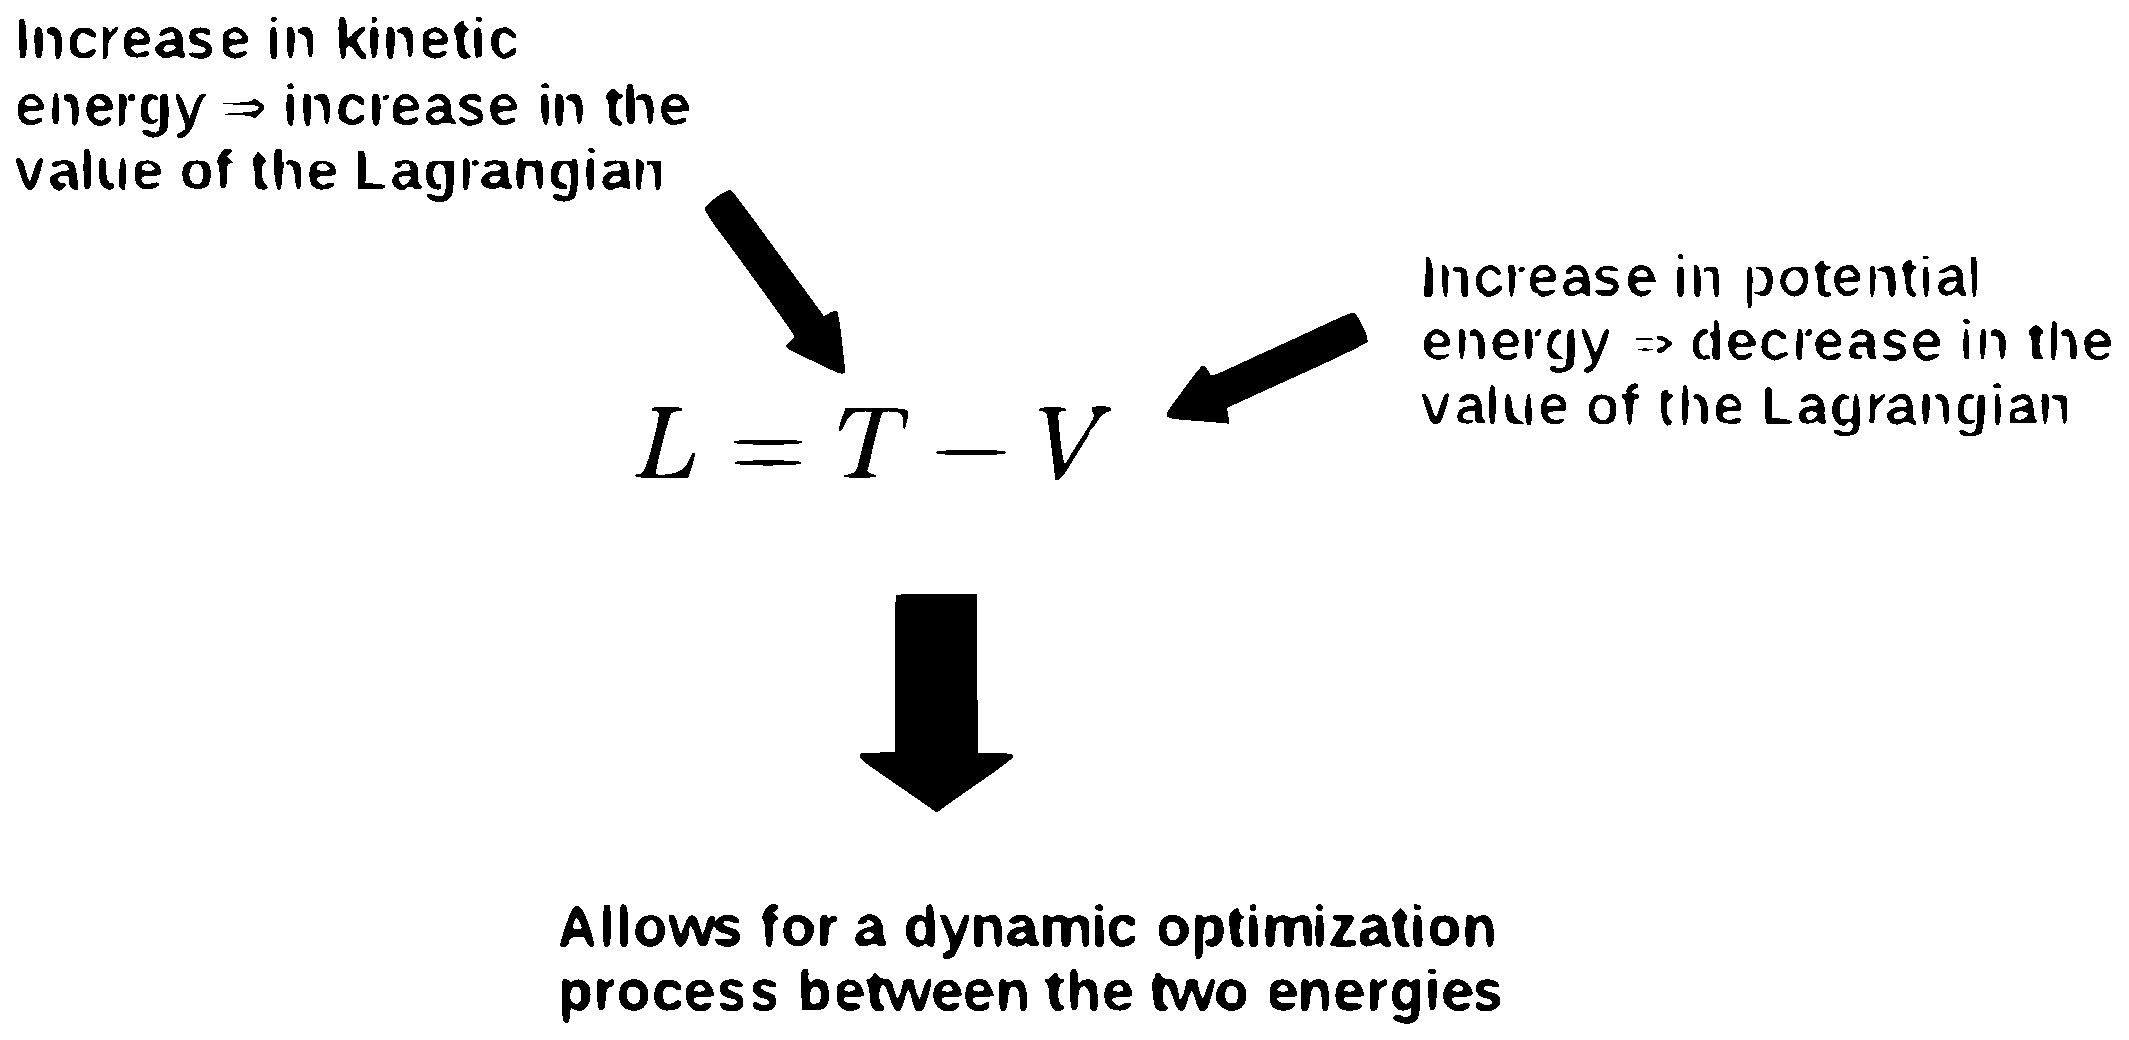
\includegraphics[width=\textwidth]{./MM21B024/image-29.eps}
        \caption{The Lagrangian Operator}
        \label{fig:my_label}
    \end{figure}
    
\section{Explanation of equation}
This is a mechanical model developed by Lagrange to analyse complex systems which are very difficult to analyse by Newtonian Mechanics. The process follows the calculus of variations and defines a procedure to analyse a system by the Euler Lagrangian equation which is a result of Hamilton's principle of least action.The mechanical state of the object i.e its potential and kinetic energies are determined in terms of generalised coordinates. The number of generalised coordinates of a body is same as the number of degrees of freedom it has.The generalised coordinates have their own velocities defined as their derivatives with respect to time. The Lagrangian is now expressed in terms of the generalised coordinates and their velocities. By principle of least action and calculus we arrive at the Euler Lagrangian equation. On proceeding to do the math we get a second order partial differential equation in the generalised coordinate. On solving all the partial differential equations simultaneously we can calculate the exact state of the system at a given time. This setup is generally used to analyse oscillators.  




